\documentclass{../exhibit}

\title{Plundered Treasure}

%% Font
\usepackage{imfellEnglish}
\usepackage[T1]{fontenc}
\raggedright

\usepackage{background}

\backgroundsetup{
scale=1,
color=black,
opacity=0.4,
angle=0,
contents={%
  \includegraphics[height=\paperheight]{mapBackground.jpg}%%https://upload.wikimedia.org/wikipedia/commons/8/81/Nautical_chart_of_the_West_Indies_1797.jpg
  }%
}




%% For the context
%% https://tex.stackexchange.com/questions/86150/torn-page-effect/86151#86151
\usepackage{tikz}
\usetikzlibrary{decorations.pathmorphing}
\definecolor{paper}{RGB}{239,227,157}





\renewcommand{\maketitle}{ %
  \begin{center}
    \scalebox{8}{\thetitle}
  \end{center}
  
\begin{tabular*}{\textwidth}{c @{\extracolsep{\fill}} c}  
\resizebox{4in}{!}{\begin{minipage}[b]{3in}\huge\directions\end{minipage}} &
  \resizebox{4in}{!}{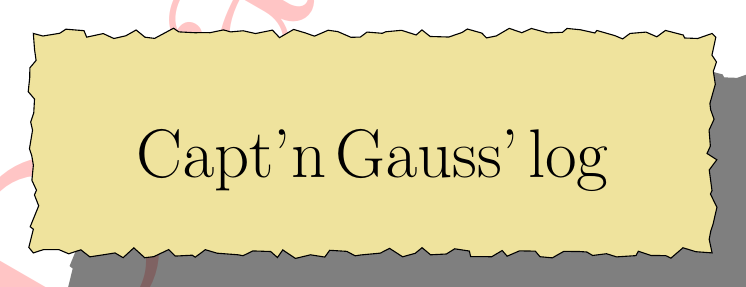
\begin{tikzpicture}[pencildraw/.style={ %
    decorate,
    decoration={random steps,segment length=4pt,amplitude=2pt}
    } %
]
\node[
preaction={fill=black,opacity=.5,transform canvas={xshift=.5cm,yshift=-.5cm}},
pencildraw,draw,fill=paper,text width=3in,inner sep=.5cm] 
{\begin{center}\Huge Capt'n Gauss' log \end{center}\vspace{.7cm} {\huge\context}};
\end{tikzpicture}}

\end{tabular*}

\vfill

\includegraphics[width=3in]{logoPirate.png}\hfill \includegraphics[width=2in]{bammLogo.png}


}


\begin{document}

\begin{context} I need your help\dots


Move all the treasure disks from


\quad ``Treasure Island''

\quad \quad \quad\quad to the


\quad \quad \quad \quad \quad ``Pirate Ship''




using the ``Port'' as a
temporary holding area.


Use the ``Port'' wisely!
\end{context}

\begin{directions}
\begin{itemize}
\item The left most tower is the ``Island.''
\item The middle post is the ``Port.''
\item The final post is the ``Ship.''
\end{itemize}

Place treasure disks on the ``Island'' tower in order with the largest
at the bottom and the smallest at the top.
\begin{itemize}
\item Move one treasure disk at a time, move it to any where you want
  BUT
\item never place a larger treasure disk on top of a smaller one.
\end{itemize}
You WIN when all the treasure is on the SHIP!
\end{directions}


\begin{example}
  The initial configuration might look like this:
\begin{center}
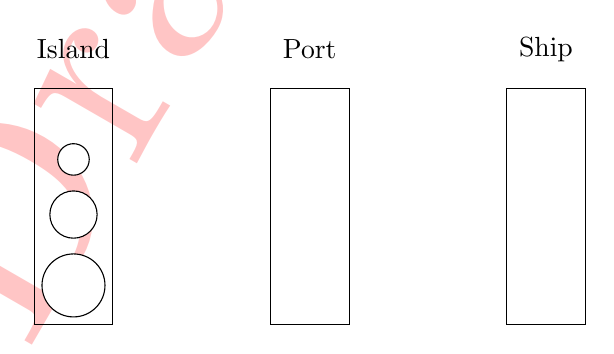
\begin{tikzpicture}
    % Draw the three towers
    \draw (0,0) -- (0,3) -- (1,3) -- (1,0) -- cycle;
    \draw (3,0) -- (3,3) -- (4,3) -- (4,0) -- cycle;
    \draw (6,0) -- (6,3) -- (7,3) -- (7,0) -- cycle;

    % Draw the disks
    \filldraw[fill=white] (0.5,2.1) circle (0.2);
    \filldraw[fill=white] (0.5,1.4) circle (0.3);
    \filldraw[fill=white] (0.5,0.5) circle (0.4);

    % Draw labels
    \node at (0.5,3.5) {Island};
    \node at (3.5,3.5) {Port};
    \node at (6.5,3.5) {Ship};
\end{tikzpicture}
\end{center}
\end{example}


\begin{mathConnections}
  https://bartsnapp.github.io/Math-Outreach-Exhibits/towersOfHanoi/
\end{mathConnections}

\end{document}
